
% This LaTeX was auto-generated from MATLAB code.
% To make changes, update the MATLAB code and republish this document.

\documentclass{article}
\usepackage{graphicx}
\usepackage{color}

\sloppy
\definecolor{lightgray}{gray}{0.5}
\setlength{\parindent}{0pt}

\begin{document}

    
    
\subsection*{Contents}

\begin{itemize}
\setlength{\itemsep}{-1ex}
   \item This Routines Demos the steps taken for all sky calibration
   \item Toggle figures on or off
   \item Step 1: Collect star catalogue
   \item Step 2: Collect information about the camera
   \item Step 3: Calculate star positions at camera location
   \item Step 4: Get Image/ FITS File or Matrix
   \item Step 5: Extract stars
   \item Step 6: Calibrate stars from camera with stars from the star chart
   \item Step 7: Rotate the initial Az-El stencil according to the above calibrated parameters
   \item Functions
   \item Calibration Function
\end{itemize}


\subsection*{This Routines Demos the steps taken for all sky calibration}

\begin{verbatim}
clear all;
\end{verbatim}


\subsection*{Toggle figures on or off}

\begin{verbatim}
toggle = 1; % ON
% toggle = 0; % OFF
\end{verbatim}


\subsection*{Step 1: Collect star catalogue}

\begin{verbatim}
starCatFITS = [initialize_root_path,filesep,'energy-height-conversion',...
    filesep,'Tools',filesep,'External Tools',filesep,...
    'skymap',filesep,'hipparcos_extended_catalogue_J2000.fit'];

stars = get_star_catalogue(starCatFITS); % Star catalogue [INPUT]
\end{verbatim}


\subsection*{Step 2: Collect information about the camera}

\begin{par}
Automatically calculating the darkest frame, so that we can use clear sky for calibration [Will be removed when converting the code to a function]
\end{par} \vspace{1em}
\begin{verbatim}
fileStr = 'C:\Users\nithin\Downloads\20080326.001_bc_15sec-full_v2.h5';
[totalIntensity,timeArr]=estimate_darkest_frame(fileStr);
[val,indx]=min(totalIntensity);
timeStr = datestr(timeArr(indx));

% Get the time of the image
time = timeArr(indx); % [INPUT]

% Get camera location
dasc.sensorLoc = h5read(fileStr,'/DASC/sensorloc'); % [INPUT]
\end{verbatim}


\subsection*{Step 3: Calculate star positions at camera location}

\begin{par}
Approximate star position is calculated using the following function
\end{par} \vspace{1em}
\begin{verbatim}
[stars.az,stars.el] = RADec2AzEl(rad2deg(stars.RA),rad2deg(stars.DEC),...
    dasc.sensorLoc(1),dasc.sensorLoc(2),datestr(time,'yyyy/mm/dd HH:MM:ss'));
\end{verbatim}
\begin{par}
Storing the location of a known star. In this case: the pole star.
\end{par} \vspace{1em}
\begin{verbatim}
polarisIndx = find(stars.HIP==11767);
% The index of polaris star in the star catalogue

polaris.az = stars.az(polarisIndx);
polaris.el = stars.el(polarisIndx);
\end{verbatim}
\begin{par}
A more accurate calculation can be made using the following function. It takes more time though.
\end{par} \vspace{1em}
\begin{verbatim}
[polaris.azAccurate,polaris.elAccurate] = get_star_az_el...
    (stars.RA(polarisIndx),stars.DEC(polarisIndx),...
    stars.pmRA(polarisIndx),stars.pmDEC(polarisIndx),stars.parallax(polarisIndx),...
    stars.RV(polarisIndx),time,deg2rad(dasc.sensorLoc(1)),deg2rad(dasc.sensorLoc(2)),dasc.sensorLoc(3));
\end{verbatim}


\subsection*{Step 4: Get Image/ FITS File or Matrix}

\begin{verbatim}
asiPath = 'C:\Users\nithin\Documents\GitHub\LargeFiles\DASC\20080326\';
asi1File = 'PKR_DASC_0000_20080326_103958.000.FITS';
image1 = fitsread([asiPath,asi1File]); %% [INPUT]
display_image(toggle,image1,[300 500],'Original Image');
\end{verbatim}

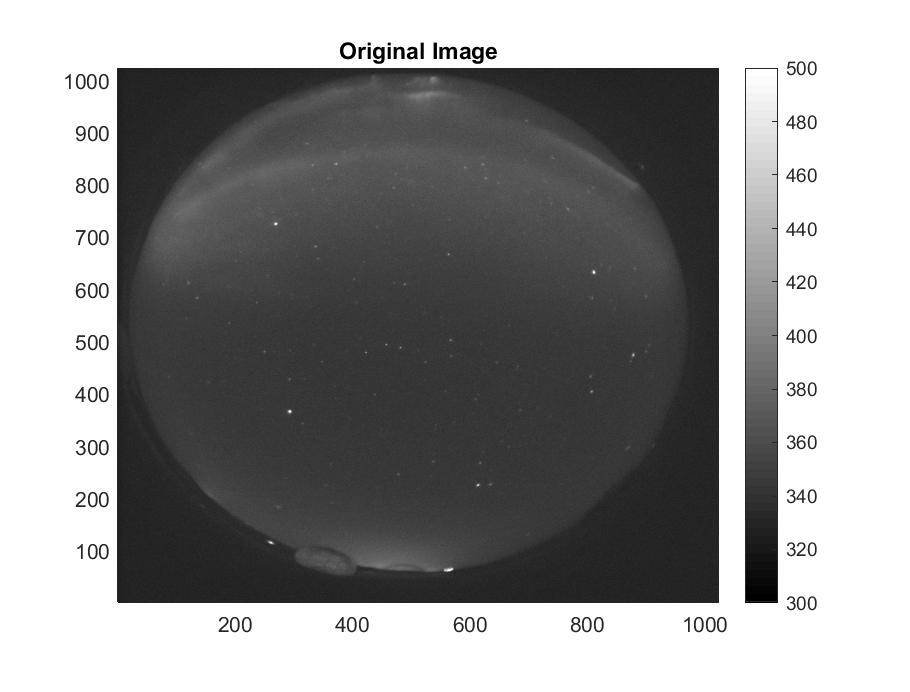
\includegraphics [width=4in]{asi_star_calibration_demo_01.eps}
\begin{par}
\texttt{Get initial azimuth elevation grid}
\end{par} \vspace{1em}
\begin{verbatim}
[dasc.az, dasc.el] = get_AzEl_grid(size(image1,1));
\end{verbatim}
\begin{par}
\textbf{Step 4.1. Remove hot pixels} If one needs to remove hot pixels one can attach another image that is separated in time
\end{par} \vspace{1em}
\begin{verbatim}
asi2File = 'PKR_DASC_0000_20080326_133018.000.FITS';
image2 = fitsread([asiPath,asi2File]);
[hotPixels] = identify_hot_pixels(image1, image2, 10);
display_image(toggle,hotPixels,[],'Hot pixles');
\end{verbatim}

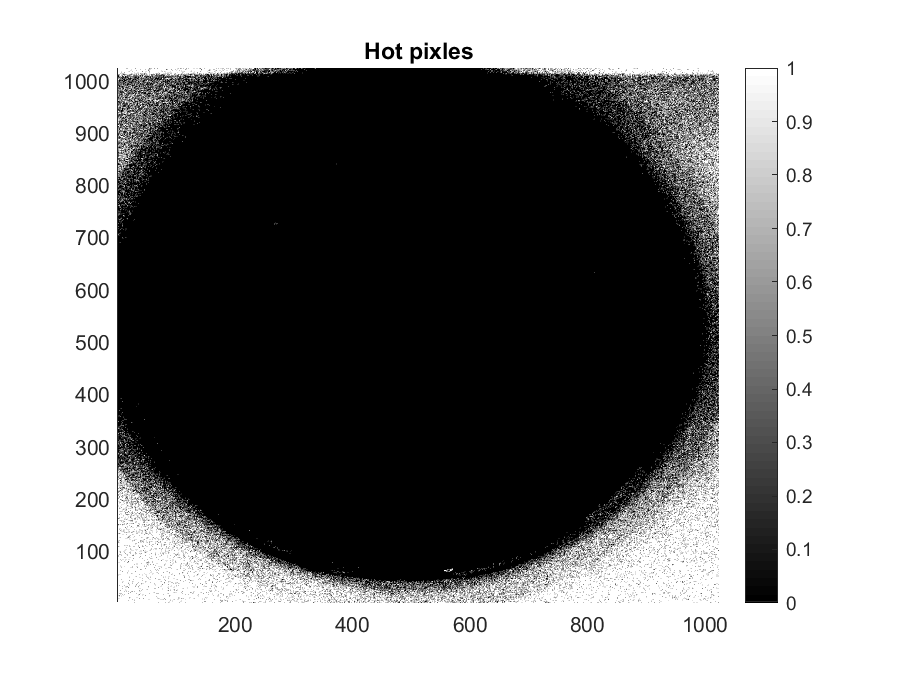
\includegraphics [width=4in]{asi_star_calibration_demo_02.eps}
\begin{par}
\textbf{Step 4.2. Remove background}
\end{par} \vspace{1em}
\begin{verbatim}
[image1BkgRem,backgroundRow, imRowNoise, pRow, muRow, a] = remove_background(image1,5);
display_image(toggle,image1BkgRem,[0 100],'Image with background removed from row');
display_image(toggle,backgroundRow, [200 800], 'Background with stars removed (After Row fits)');
display_image(toggle,imRowNoise,[0 10],'Noise (row fit)');

[image1BkgRem,background1, imColNoise] = remove_background(image1BkgRem');
image1BkgRem = image1BkgRem';
imColNoise = imColNoise';
background1 = background1'; %Background of the image i.e. without the stars.
display_image(toggle, image1BkgRem, [0 100], 'Image with background removed from row and column');
display_image(toggle,background1, [0 50], 'Background with stars removed (After Row and Col fits)');
display_image(toggle,imColNoise,[0 10],'Noise (col fit)');
\end{verbatim}

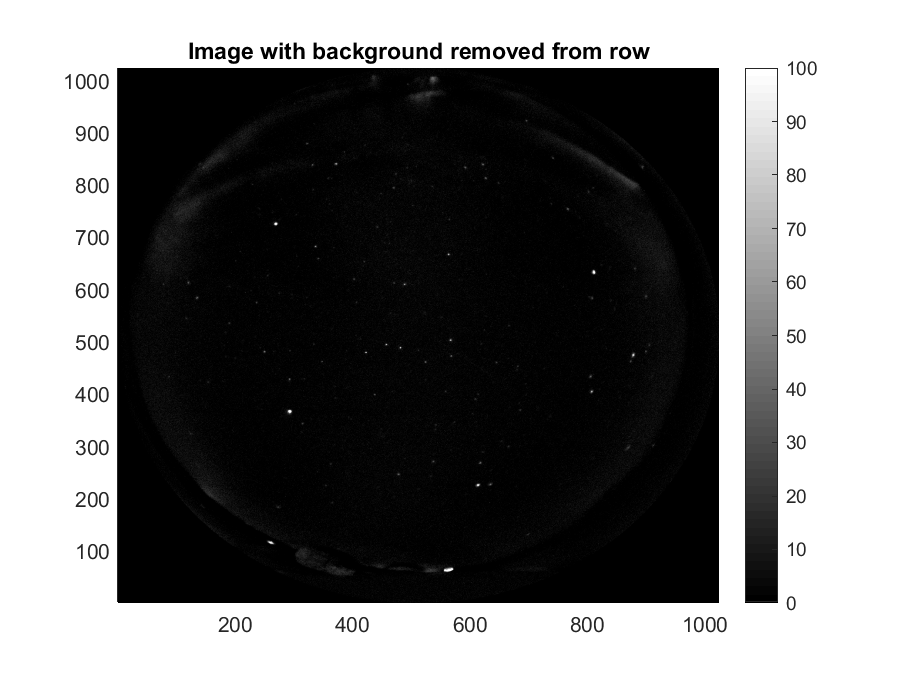
\includegraphics [width=4in]{asi_star_calibration_demo_03.eps}

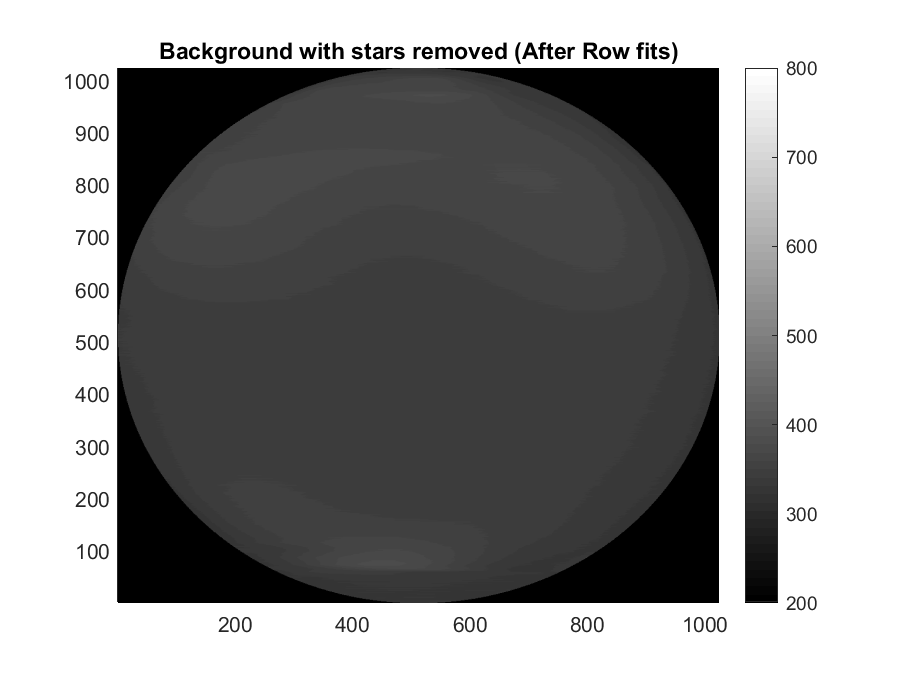
\includegraphics [width=4in]{asi_star_calibration_demo_04.eps}

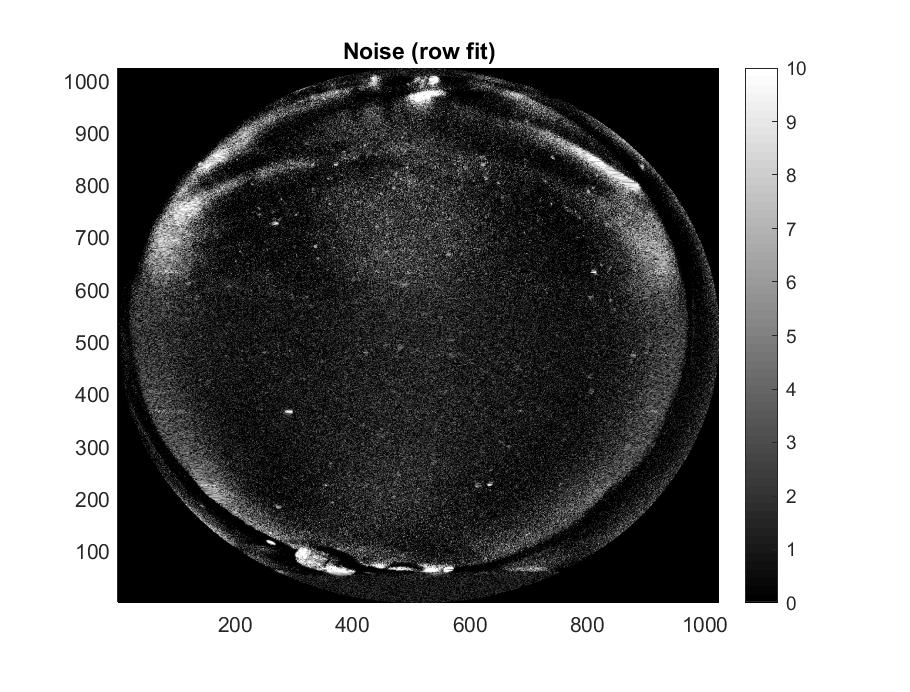
\includegraphics [width=4in]{asi_star_calibration_demo_05.eps}

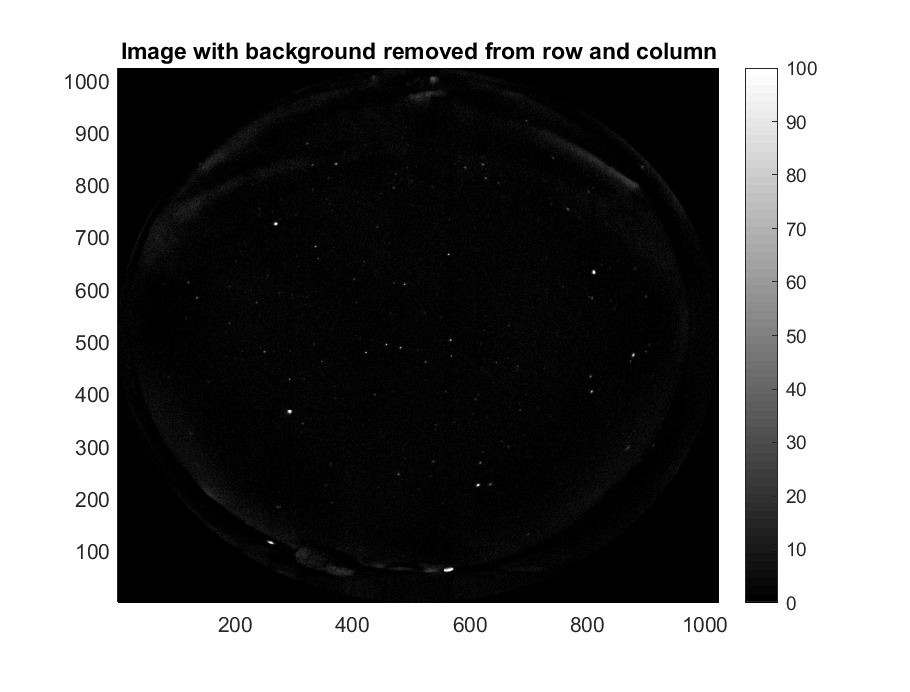
\includegraphics [width=4in]{asi_star_calibration_demo_06.eps}

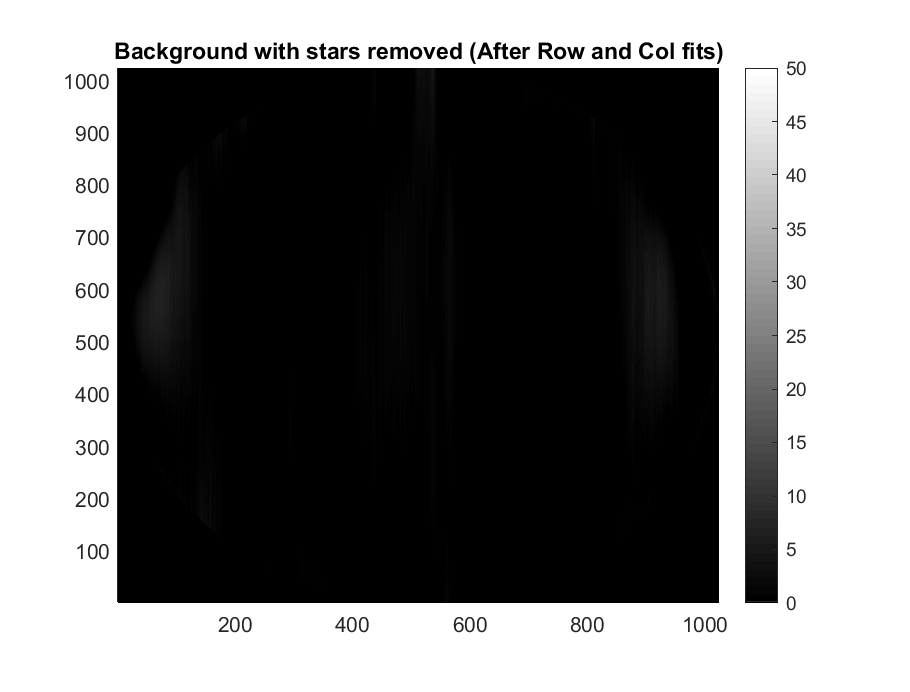
\includegraphics [width=4in]{asi_star_calibration_demo_07.eps}

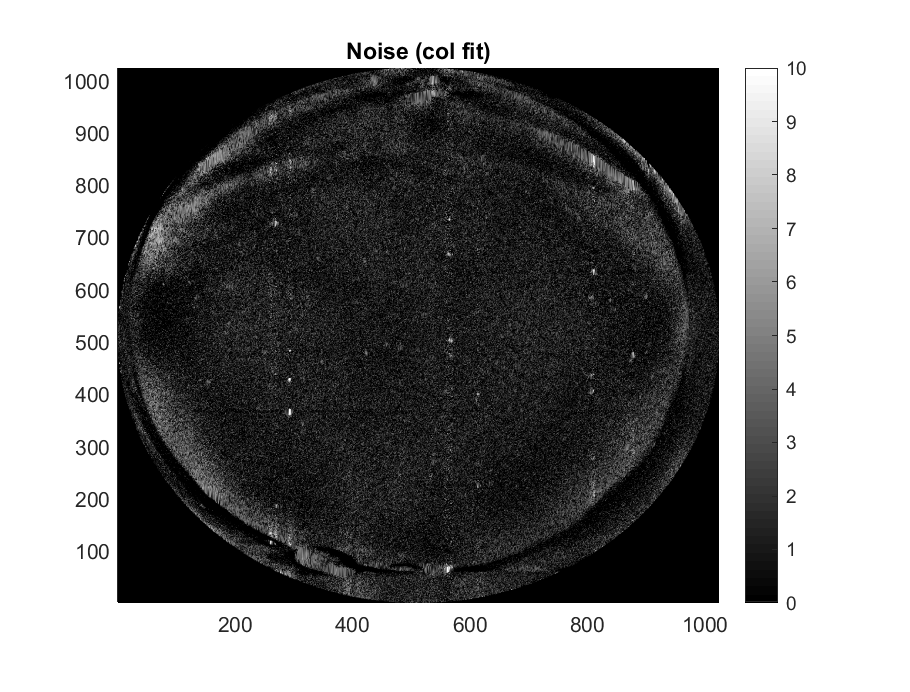
\includegraphics [width=4in]{asi_star_calibration_demo_08.eps}
\begin{par}
\textbf{Step 4.3. Calculate noise at each pixel}
\end{par} \vspace{1em}
\begin{verbatim}
fnoise = @(x) nanstd(x(:));
totalNoise = imColNoise+imRowNoise;
totalNoise(totalNoise==0)=nan;
sigma_n = nlfilter(totalNoise,[9 9],fnoise); % calculating std deviation from neighbouring pixels!
display_image(toggle, sigma_n, [0 10], '\sigma_n Noise at each pixel');
\end{verbatim}

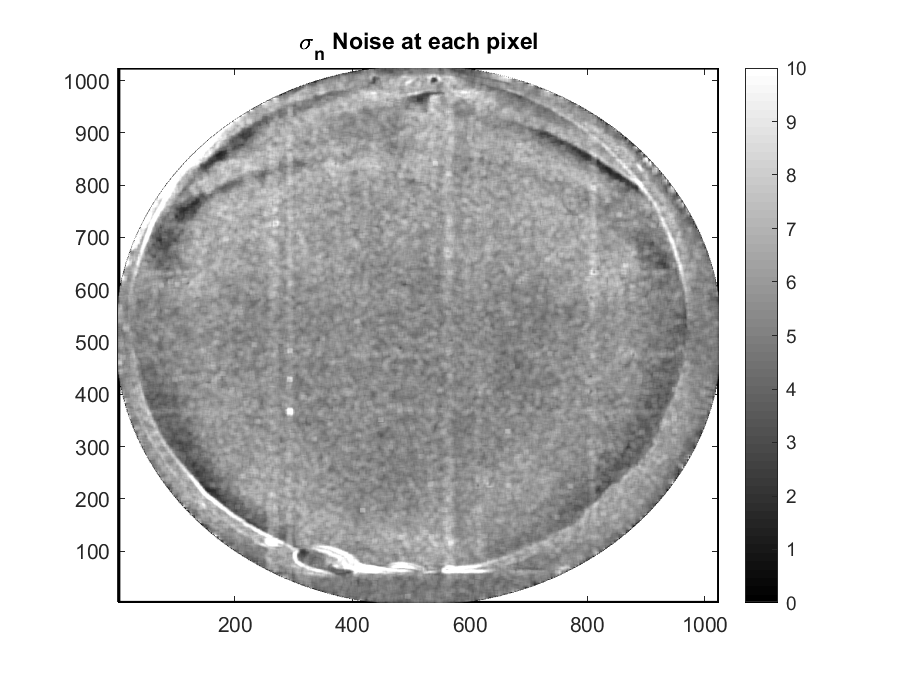
\includegraphics [width=4in]{asi_star_calibration_demo_09.eps}
\begin{par}
\textbf{Step 4.4. Removing noise spikes}
\end{par} \vspace{1em}
\begin{verbatim}
image1NoiseRem = remove_noise_spikes(image1BkgRem, sigma_n);
display_image(toggle, image1NoiseRem, [0 100], 'Image with bkg and noise removed');
\end{verbatim}

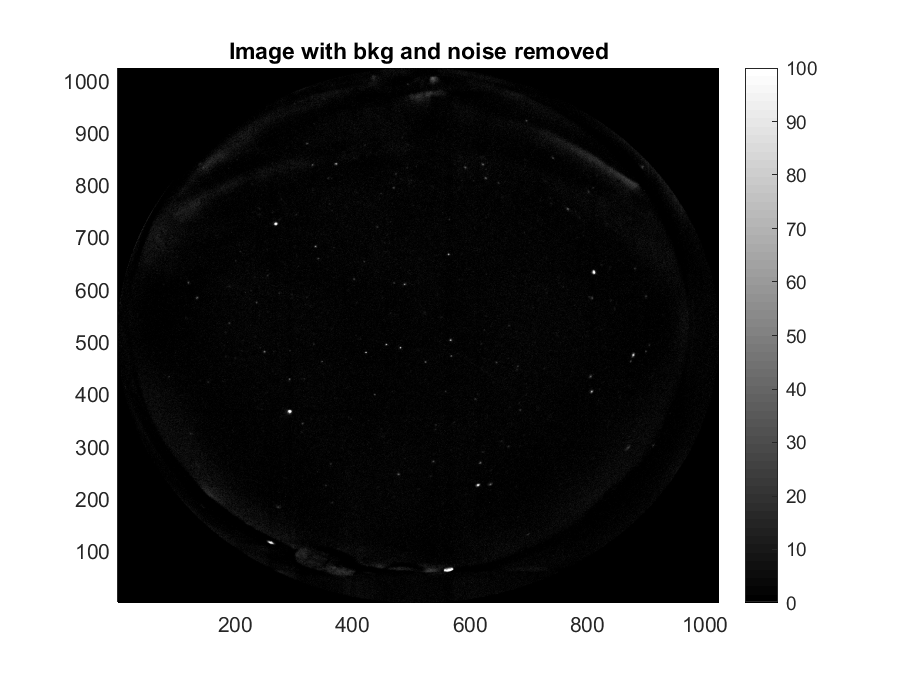
\includegraphics [width=4in]{asi_star_calibration_demo_10.eps}
\begin{par}
\textbf{Step 4.5. Removing hot pixels} See step 4.1
\end{par} \vspace{1em}
\begin{verbatim}
image1BkgRem(logical(hotPixels(:)))= nan;
\end{verbatim}


\subsection*{Step 5: Extract stars}

\begin{verbatim}
starImage = faint_star_extracter(image1BkgRem, sigma_n);
starImage(starImage <= 20) = 0;
\end{verbatim}

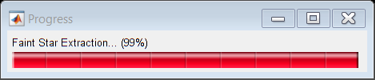
\includegraphics [width=4in]{asi_star_calibration_demo_11.png}
\begin{verbatim}
display_image(toggle, starImage, [0 100], 'Stars extracted');
\end{verbatim}

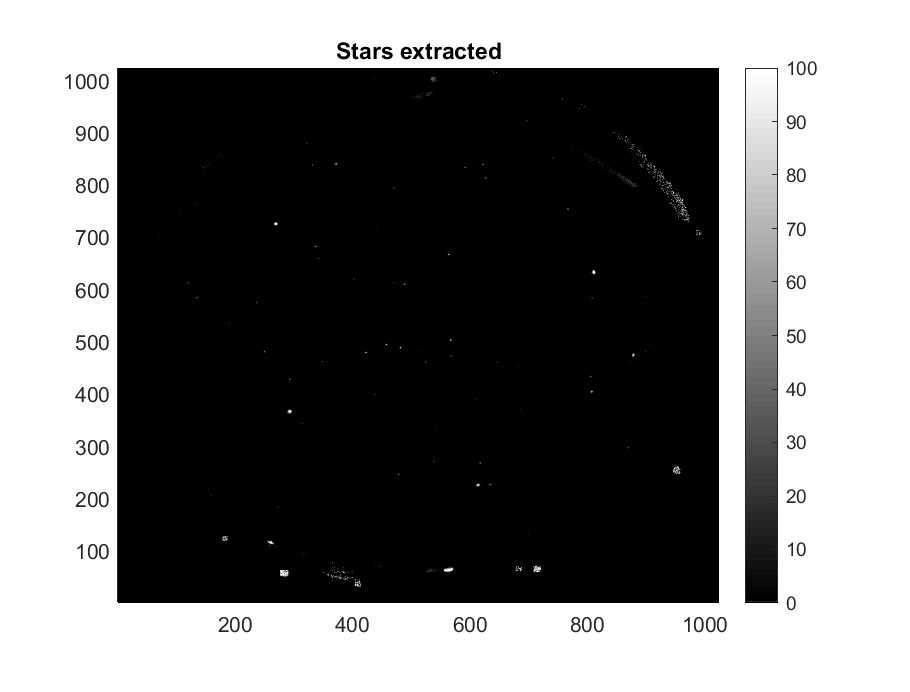
\includegraphics [width=4in]{asi_star_calibration_demo_12.eps}
\begin{par}
\textbf{Step 5.1. Extract stars}
\end{par} \vspace{1em}
\begin{verbatim}
imstarStruct = extract_stars(starImage);
dascstar = filter_stars(imstarStruct, 22.5); % remove points in the corners of the image
if toggle == 1
    hold on;
    scatter(dascstar.location(:,1), dascstar.location(:,2),20*dascstar.brightness, 'r');
    legend('Extracted stars', 'Centroid');
end
\end{verbatim}

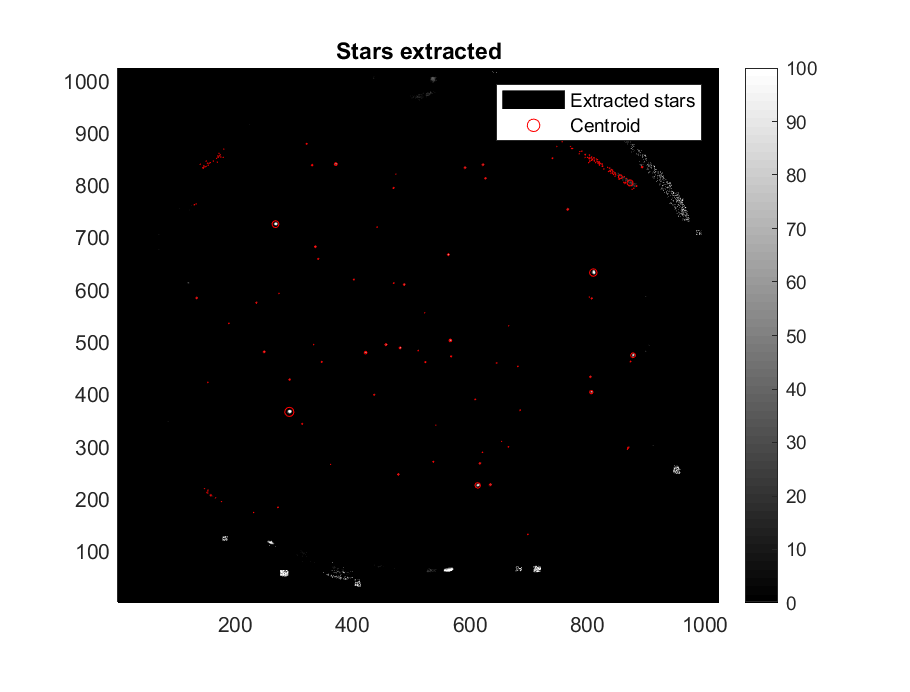
\includegraphics [width=4in]{asi_star_calibration_demo_13.eps}
\begin{par}
\textbf{Step 5.2. Get real stars in the above format}
\end{par} \vspace{1em}
\begin{verbatim}
realstar = get_actual_stars(stars, 22.5, 4, 0, 0, 0, 1);
\end{verbatim}


\subsection*{Step 6: Calibrate stars from camera with stars from the star chart}

\begin{verbatim}
[dascstarCal,calPar,fval,acc] = calibrate_stars(realstar,dascstar,dasc.az, dasc.el);
\end{verbatim}
\begin{verbatim}
if toggle == 1
    figure;
    plot_aer_stars(realstar.locationAzEl(:,1), realstar.locationAzEl(:,2),...
        realstar.brightness*50, 'r', 0, 0, 0, 1, 0);
    hold on;
    plot_aer_stars(dascstarCal.locationAzEl(:,1), dascstarCal.locationAzEl(:,2),...
        dascstarCal.brightness*50, 'c',...
        calPar(1), calPar(2), calPar(3), calPar(4), calPar(5), calPar(6));
    legend('Star chart','From calibrated parameters');
end
\end{verbatim}

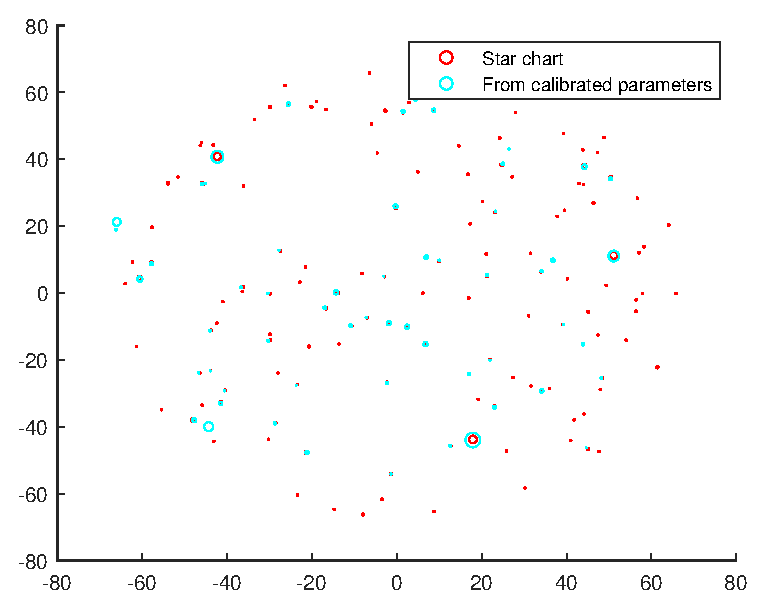
\includegraphics [width=4in]{asi_star_calibration_demo_14.eps}
\begin{par}
Step 6.1: Transform the stars identified from image to new Az El values
\end{par} \vspace{1em}
\begin{verbatim}
[dascStarAz, dascStarEl] = calculate_new_AzEl(dascstarCal.locationAzEl(:,1),...
    dascstarCal.locationAzEl(:,2),calPar);
if toggle == 1
    hold on;
    plot_aer_stars(dascStarAz, dascStarEl, dascstarCal.brightness*30, 'g', 0, 0, 0, 1);
    legend('From star chart','From calibrated parameters','From new az-el grid');
end
\end{verbatim}

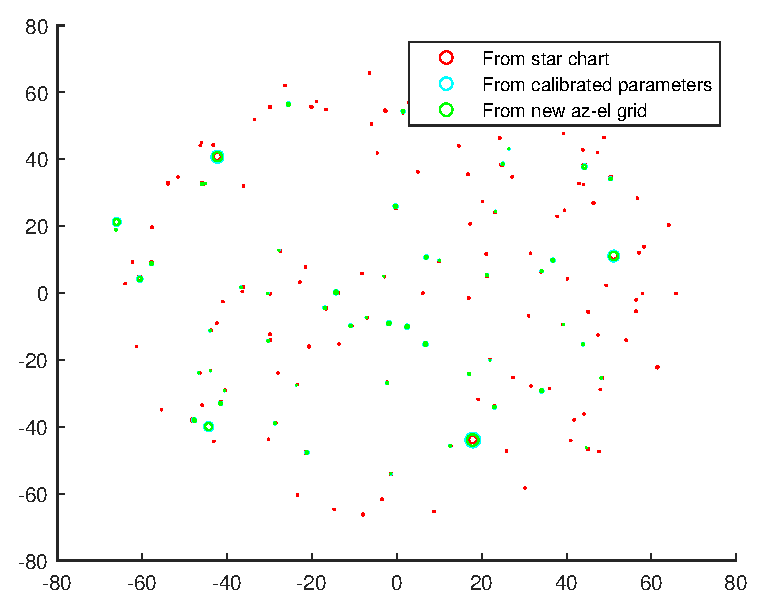
\includegraphics [width=4in]{asi_star_calibration_demo_15.eps}


\subsection*{Step 7: Rotate the initial Az-El stencil according to the above calibrated parameters}

\begin{verbatim}
[dasc.azCal, dasc.elCal] = calculate_new_AzEl(dasc.az,dasc.el,calPar);

if toggle == 1
    indx = dasc.elCal>0;
    h = figure;
    resize_figure(h,300,300);
    dsign = -1;
    p(1) = plot_DASC_aer(image1(indx), dasc.azCal(indx), dasc.elCal(indx), 1024, dsign);
    colorbar;
    colormap('viridis');
    xlim([-120,+120]);
    ylim([-120,+120]);
    hold on;
    p(2) = plot_aer_stars(realstar.locationAzEl(:,1), realstar.locationAzEl(:,2),...
        realstar.brightness*80, 'c', 0, 0, 0, dsign);
    hold on;
    p(3) = plot_aer_stars(dascStarAz, dascStarEl, dascstarCal.brightness*50, 'r', 0, 0, 0, dsign);

    hold on;
    plot_grid_aer([0, 90], 22.5, 'm');
    caxis([300 450]);

    hold on;
    plot_star_names(realstar, 8, 'w', 0, 0, 0, dsign);
    legend([p(1), p(2), p(3)], 'Calibrated image','Star chart','Stars from calibrated grid');
    title(timeStr);
    accuracy = (median(min(pdist2([dascStarAz,dascStarEl],...
        realstar.locationAzEl(1:length(dascStarAz),:)))));
    text(-90,-90,['Accuracy : ~',...
        num2str(accuracy,2),'�']);
end
\end{verbatim}


\subsection*{Functions}

\begin{verbatim}
function [totalIntensity,timeArr]=estimate_darkest_frame(h5FileStr)

asi = permute(h5read(h5FileStr,'/DASC/ASI'),[3 2 1]);
timeArr = unixtime2matlab((h5read(h5FileStr,'/DASC/time'))');
totalIntensity = sum(sum(asi,3),2);

end
\end{verbatim}
\begin{verbatim}
function display_image(toggle,image,clim,titleStr)

if toggle==1

    if nargin<4
        titleStr = '';
    end

    figure;
    h=pcolor(image);
    set(h,'EdgeColor','none');
    colorbar;
    colormap(get_colormap('k','w'))
    title(titleStr);

    if ~(nargin<3) && ~isempty(clim)
        caxis(clim);
    end
end

end
\end{verbatim}
\begin{verbatim}
function [hotPixels] = identify_hot_pixels(image1, image2, threshold)

if nargin<3
    threshold = 2;
end

temp = image1 - image2;
temp2 = temp;
hotPixels=zeros(size(temp2));
hotPixels(abs(temp2)<=threshold) = 1;
end
\end{verbatim}
\begin{verbatim}
function [ASINew, background, ASINoise, pRow, muRow, a] = remove_background(ASI, nPoly)

% Remove background along the row

if nargin < 2
    nPoly = 3;
end

% ASINew, background
rowIndx = 1:1:size(ASI,2);
colIndx = 1:1:size(ASI,1);
ASINew = zeros(size(ASI));
background = zeros(size(ASI));
ASItemp = ASI;
ASINoise = zeros(size(ASI));
pRow = zeros([length(rowIndx),nPoly+1]);
% First iteration
for ifit = 1:2
    for i = rowIndx
        lchord = sqrt(512.^2-(abs(512-i)).^2);
        fitRangeIndx =512-round(lchord)+1:1:512+round(lchord);
        x = colIndx(fitRangeIndx);
        y = ASItemp(i,fitRangeIndx);
        if length(fitRangeIndx)>10
            pRow(i,:)=polyfit(x,y,nPoly);
        end
        muRow(i,:)=mean(y);
        stdRow(i,:) = std(y);
        a(i).fitRangeIndx = fitRangeIndx;
        background(i,fitRangeIndx) = polyval(pRow(i,:),colIndx(fitRangeIndx));
        if ifit==1
            brightStarIndx = ASItemp(i,:) > (background(i,:)+1*stdRow(i,:));
            if ~isempty(find(brightStarIndx)>0)
                ASItemp(i,brightStarIndx) = nan;
                ASItemp(i,fitRangeIndx) = interp_nans(ASItemp(i,fitRangeIndx)')';
            end
        else
            ASINew(i,fitRangeIndx) = ASI(i,fitRangeIndx)-background(i,fitRangeIndx);
            ASINoise(i,fitRangeIndx) = ASItemp(i,fitRangeIndx)-background(i,fitRangeIndx);
        end

    end
end

end
\end{verbatim}

        \color{lightgray} \begin{verbatim}Warning: Polynomial is badly conditioned. Add
points with distinct X values, reduce the degree of
the polynomial, or try centering and scaling as
...\end{verbatim} \color{black}
    \begin{verbatim}
function ASI = remove_noise_spikes(ASI, sigma_n)

for i=3:1:size(ASI,1) - 2
    for j = 3:1:size(ASI,2) - 2
        A = ASI(i,j);
        B1 = ASI(i,j-1);    B2 = ASI(i,j-2);
        C1 = ASI(i-1,j);    C2 = ASI(i-2,j);
        D1 = ASI(i,j+1);    D2 = ASI(i,j+2);
        E1 = ASI(i+1,j);    E2 = ASI(i+2,j);
        s = sigma_n(i,j);
        singleSpike = (A > 2*s)*(B1 < 2*s)*(C1 < 2*s)*(D1 < 2*s)*(E1 < 2*s);
        doubleSpike(1) = (A > 3*s)*((B1>2*s)*(B2<2*s))*...
            not((C1>2*s))*not((D1>2*s))*...
            not((E1>2*s));
        doubleSpike(2) = (A > 3*s)*not((B1>2*s))*...
            ((C1>2*s)*(C2<2*s))*not((D1>2*s))*...
            not((E1>2*s));
        doubleSpike(3) = (A > 3*s)*not((B1>2*s))*...
            not((C1>2*s))*((D1>2*s)*(D2<2*s))*...
            not((E1>2*s));
        doubleSpike(4) = (A > 3*s)*not((B1>2*s))*...
            not((C1>2*s))*not((D1>2*s))*...
            ((E1>2*s)*(E2<2*s));
        ASI(i,j) = not(singleSpike).*A;
        ASI(i,j) = not(sum(doubleSpike)).*A;
        ASI(i,j-1) = not(doubleSpike(1)).*B1;
        ASI(i-1,j) = not(doubleSpike(2)).*C1;
        ASI(i,j+1) = not(doubleSpike(3)).*D1;
        ASI(i+1,j) = not(doubleSpike(4)).*E1;
    end
end


end
\end{verbatim}
\begin{verbatim}
function [starImage] = faint_star_extracter(ASI, sigma_n)

mSz = 7;
MSz = 9;
dSz = (MSz-mSz)/2;
if mod(dSz,1)
    error('mSz-MSz has to be even');
end

starImage = zeros(size(ASI));

multiWaitbar('Faint Star Extraction...',0);
id = 1./size(ASI,1);
% For faint stars
for i=1:1:size(ASI,1) - MSz
    for j = 1:1:size(ASI,2) - MSz
        M = ASI(i:i+MSz-1,j:j+MSz-1);
        in = M(1+dSz:dSz+mSz,1+dSz:dSz+mSz);
        out = M;
        out(1+dSz:dSz+mSz,1+dSz:dSz+mSz)=0;
        sig_n = sigma_n(i+dSz+ceil(mSz/2),j+dSz+ceil(mSz/2));
        mu_in = nanmean(in(:));
        mu_out = nanmean(out(:));
        % Condition
        if mu_in > 1*sig_n && mu_out < 2*sig_n
            starImage(i:i+MSz-1,j:j+MSz-1) = M;
        end

    end
    multiWaitbar('Faint Star Extraction...','Increment',id);
end

end
\end{verbatim}
\begin{verbatim}
function imstar = extract_stars(image)
% Image should be post all processing
binaryImage = zeros(size(image));
binaryImage(image>0)=1;
[labelImage, numSpots] = bwlabel(binaryImage);
props = regionprops(labelImage,image,'Centroid','Area','MeanIntensity');
for i =1:1:numSpots
    imstar.ID(i,1) = i;
    imstar.location(i,:) = props(i).Centroid;
    imstar.brightness(i,1) = props(i).Area.*props(i).MeanIntensity;
end
imstar.brightness = imstar.brightness./max(imstar.brightness); % Relative magnitude
imstar.size = size(image);
end
\end{verbatim}
\begin{verbatim}
function [newstar, I] = filter_stars(imstar, elMax, astrometryFileStr)
% Function sorts stars according to brightness, and defines a FoV of
% interest.

% Input
% imstar: A structure of star extracted from image
% elMax : Stars below this elevation will not be considered
% astrometryFileStr : A text file written in the format necessary
%                     for astrometry web utility: http://nova.astrometry.net/upload

% Output
% newstar: A structure with stars sorted according to intensity
% I      : Sorting index

if nargin<3
    astrometryFileStr = []; % File containing text that can uploaded to astrometry
end
% Restricting the field of view.
FOV  = (90-elMax)*2;
% Assuming fish eye
imLength = imstar.size(1);
LengthperElevation = imLength/180;
p.min = round(imLength/2) - round(LengthperElevation*FOV/2);
p.max = round(imLength/2) + round(LengthperElevation*FOV/2);

selectedStarIndx =(imstar.location(:,1)>p.min &...
    imstar.location(:,1)<p.max & ...
    imstar.location(:,2)>p.min & ...
    imstar.location(:,2)<p.max);

newstar.location = imstar.location(selectedStarIndx,:);
newstar.brightness = imstar.brightness(selectedStarIndx)';

% Sorting the stars based on its magnitude.
[newstar, I] = sort_star(newstar);

if ~isempty(astrometryFileStr)
    dlmwrite(astrometryFileStr,round(newstar.location));
end

end
\end{verbatim}
\begin{verbatim}
function [newstar, I] = sort_star(newstar)
% Function that sorts stars according to brightness
[newstar.brightness, I] = sort(newstar.brightness,'descend');
newstar.brightness = newstar.brightness';
newstar.location = newstar.location(I,:);
end

function realstar = get_actual_stars(stars,elCutOff,magCutOff,dx,dy,drot, dsign)
if nargin < 7
    dsign = 1;
end

starfilter=stars.vmag<magCutOff & stars.el>elCutOff;
[x,y] = get_aer_stars(stars.az(starfilter), stars.el(starfilter), dx, dy, drot, dsign);
realstar.location = [x, y]; %pixel location
realstar.brightness = stars.relIntensity(starfilter);
realstar.locationAzEl = [stars.az(starfilter), stars.el(starfilter)];
realstar.name = stars.name(starfilter);
[realstar, I] = sort_star(realstar); %s
realstar.locationAzEl = realstar.locationAzEl(I,:);
realstar.name = realstar.name(I);
end
\end{verbatim}
\begin{verbatim}
function [x,y] = get_aer_stars(az, el, dx, dy, drot, dsign, dr, k, k0)
if nargin <9
    k0 = 0; % k0 is an unused parameter.
end
if nargin <8
    k = 0; % k is the distortion parameter
end
if nargin <7
    dr = 0; % Determines the field of view in the image
end
if nargin<6
    dsign = 1;
end
az = rotate_array(az,drot);

% r1 = (90-el);
r0 = (90-el);
k = 1+k.*10^-6;
r1 = (90.^((k-1)./k)).*r0.^(1./k);

r = r1 + dr.*r1;
x = dx + dsign.*((r).*sind(az));
y = dy + (r).*cosd(az);
end
\end{verbatim}

        \color{lightgray} \begin{verbatim}Optimization terminated: average change in the fitness value less than options.FunctionTolerance.
Optimization terminated: average change in the fitness value less than options.FunctionTolerance.
Optimization terminated: average change in the fitness value less than options.FunctionTolerance.
\end{verbatim} \color{black}
    

\subsection*{Calibration Function}

\begin{par}
See \begin{verbatim}execution\end{verbatim}
\end{par} \vspace{1em}
\begin{verbatim}
function [dascstar,x,fval,accuracy] = calibrate_stars(realstar,dascstar,azOld,elOld)
dloc = round(dascstar.location);
dascstar.brightness = dascstar.brightness./max(dascstar.brightness);
lindx = sub2ind(size(azOld),dloc(:,2),dloc(:,1));
%                            rows(y)   cols(x)
dascstar.locationAzEl = [azOld(lindx), elOld(lindx)];
minElFilter = find(dascstar.locationAzEl(:,2)>=22.5);
dascstar.locationAzEl = dascstar.locationAzEl(minElFilter,:);
dascstar.brightness = dascstar.brightness(minElFilter);
dascstar.location = dascstar.location(minElFilter,:);
ndasc = length(dascstar.brightness);
starIndx = true(1,ndasc);

% dx, dy translation of center point
% drot - rotation along azimuth
% dr - is field of view (radius)
% k - radial distortion coefficient
%     dx   dy   drot    dr     k =0  k0
lb = [-10, -10, -180,  -0.1,    -100];
ub = [+10, +10, +180,  +0.1,    100];
nvars = 6;
options = optimoptions('ga');
%,'MaxGenerations',2000,'MaxStallGenerations',500
dsign = [-1, +1];
for k = 1:2
    [y(k,:),fval(k),exitflag] = ga(@starDistance,nvars,[],[],[],[],...
        lb,ub,[],options);
end

[~,minIndx] = min(fval);
x = [y(minIndx,1), y(minIndx,2), y(minIndx,3), dsign(minIndx),...
    y(minIndx,4), y(minIndx,5)];

% Removing planets and other objects not in the star database
[x2, y2] = get_aer_stars(dascstar.locationAzEl(:,1),...
    dascstar.locationAzEl(:,2),x(1),x(2),x(3),x(4),x(5),x(6));
D2 = pdist2([x2, y2], realstar.location(1:ndasc,:));
dmin2 = min(D2');
unmatchedObjects = dmin2 > 0.5; %Objects do not match if greater than 1 deg off
nMatched = sum(~unmatchedObjects);
accuracy = median(dmin2);
if nMatched>10 && accuracy<1
    starIndx = ~unmatchedObjects;
    k = minIndx;
    [y2, fval(3), ~] = ga(@starDistance,nvars,[],[],[],[],...
        lb,ub,[],options);
    if fval(3)<fval(minIndx)
        x = [y2(1,1), y2(1,2), y2(1,3), dsign(minIndx), y2(1,4), y2(1,5)];
    end
else
    if nMatched<10
    disp(['Number of stars available should be more than 10. N = ',...
        num2str(nMatched),'. Redoing the calculation']);
    end
    if accuracy>1
        disp(['Accuracy is not good enough, it is ~ ', num2str(accuracy,2),...
            '. Redoing the calculation']);
    end
    [dascstar,x,fval] = calibrate_stars(realstar,dascstar,azOld,elOld);
end

    function dmin=starDistance(x)
        [x1,y1] = get_aer_stars(dascstar.locationAzEl(starIndx,1),...
            dascstar.locationAzEl(starIndx,2),x(1),x(2),x(3),dsign(k),x(4));
        dascstar.newxy = [x1,y1];
        D = pdist2(dascstar.newxy,realstar.location(1:sum(starIndx),:));
        dmin = sum(min(D));
    end

end
\end{verbatim}
\begin{verbatim}
function [azNew, elNew] = calculate_new_AzEl(azOld,elOld,x)

[xNew,yNew] = get_aer_stars(azOld,elOld,x(1),x(2),x(3),x(4),x(5),x(6));
azNew = wrapTo360(atan2d(xNew,yNew));
elNew = 90 - xNew./(sind(azNew));
indx = elNew<=0;
azNew(indx) = nan;
elNew(indx) = nan;

end
\end{verbatim}

\includegraphics [width=4in]{asi_star_calibration_demo_16.eps}
\begin{verbatim}
function p = plot_aer_stars(az,el,relIntensity,colorStr, dx, dy, drot, dsign, dr, k, k0)

if nargin<11
    k0 = 0; %radial distortion
end
if nargin<10
    k = 0; %radial distortion
end
if nargin<9
    dr = 0; % Extent of the radius/ FoV
end
if nargin<8
    dsign = 1;
end

[x,y] = get_aer_stars(az, el, dx, dy, drot, dsign, dr, k, k0);
p = scatter(x,y,relIntensity,colorStr);

end
\end{verbatim}

\includegraphics [width=4in]{asi_star_calibration_demo_17.eps}
\begin{verbatim}
function plot_star_names(sortedStars, n, color, dx, dy, drot ,dsign)

if nargin < 3 || isempty(color)
    color = 'c';
end
if nargin <2 || isempty(n)
    n = 5;
end

hold on;

starNames = string(extractBetween((sortedStars.name(1:1:n)),'(',')'));

for i = 1:1:n
    [x,y] = get_aer_stars(sortedStars.locationAzEl(i,1), sortedStars.locationAzEl(i,2),...
        dx,dy,drot,dsign);
    t=text(x,y,strcat("  ",starNames(i)));
    t.Color = color;
    t.FontSize = 7;
end

end
\end{verbatim}

\includegraphics [width=4in]{asi_star_calibration_demo_18.eps}
\begin{verbatim}
function [az, el] = get_AzEl_grid(imageSize)

x = linspace(-90,90,imageSize);
y = linspace(-90,90,imageSize);

[X, Y] = meshgrid(x,y);

az = wrapTo360(atan2d(X,Y));
el = 90 - X./(sind(az));

indx = el<=0;
az(indx) = nan;
el(indx) = nan;

end
\end{verbatim}



\end{document}
    
